% Options for packages loaded elsewhere
\PassOptionsToPackage{unicode}{hyperref}
\PassOptionsToPackage{hyphens}{url}
\PassOptionsToPackage{dvipsnames,svgnames,x11names}{xcolor}
%
\documentclass[
  letterpaper,
  DIV=11,
  numbers=noendperiod]{scrartcl}

\usepackage{amsmath,amssymb}
\usepackage{iftex}
\ifPDFTeX
  \usepackage[T1]{fontenc}
  \usepackage[utf8]{inputenc}
  \usepackage{textcomp} % provide euro and other symbols
\else % if luatex or xetex
  \usepackage{unicode-math}
  \defaultfontfeatures{Scale=MatchLowercase}
  \defaultfontfeatures[\rmfamily]{Ligatures=TeX,Scale=1}
\fi
\usepackage{lmodern}
\ifPDFTeX\else  
    % xetex/luatex font selection
\fi
% Use upquote if available, for straight quotes in verbatim environments
\IfFileExists{upquote.sty}{\usepackage{upquote}}{}
\IfFileExists{microtype.sty}{% use microtype if available
  \usepackage[]{microtype}
  \UseMicrotypeSet[protrusion]{basicmath} % disable protrusion for tt fonts
}{}
\makeatletter
\@ifundefined{KOMAClassName}{% if non-KOMA class
  \IfFileExists{parskip.sty}{%
    \usepackage{parskip}
  }{% else
    \setlength{\parindent}{0pt}
    \setlength{\parskip}{6pt plus 2pt minus 1pt}}
}{% if KOMA class
  \KOMAoptions{parskip=half}}
\makeatother
\usepackage{xcolor}
\setlength{\emergencystretch}{3em} % prevent overfull lines
\setcounter{secnumdepth}{5}
% Make \paragraph and \subparagraph free-standing
\ifx\paragraph\undefined\else
  \let\oldparagraph\paragraph
  \renewcommand{\paragraph}[1]{\oldparagraph{#1}\mbox{}}
\fi
\ifx\subparagraph\undefined\else
  \let\oldsubparagraph\subparagraph
  \renewcommand{\subparagraph}[1]{\oldsubparagraph{#1}\mbox{}}
\fi


\providecommand{\tightlist}{%
  \setlength{\itemsep}{0pt}\setlength{\parskip}{0pt}}\usepackage{longtable,booktabs,array}
\usepackage{calc} % for calculating minipage widths
% Correct order of tables after \paragraph or \subparagraph
\usepackage{etoolbox}
\makeatletter
\patchcmd\longtable{\par}{\if@noskipsec\mbox{}\fi\par}{}{}
\makeatother
% Allow footnotes in longtable head/foot
\IfFileExists{footnotehyper.sty}{\usepackage{footnotehyper}}{\usepackage{footnote}}
\makesavenoteenv{longtable}
\usepackage{graphicx}
\makeatletter
\def\maxwidth{\ifdim\Gin@nat@width>\linewidth\linewidth\else\Gin@nat@width\fi}
\def\maxheight{\ifdim\Gin@nat@height>\textheight\textheight\else\Gin@nat@height\fi}
\makeatother
% Scale images if necessary, so that they will not overflow the page
% margins by default, and it is still possible to overwrite the defaults
% using explicit options in \includegraphics[width, height, ...]{}
\setkeys{Gin}{width=\maxwidth,height=\maxheight,keepaspectratio}
% Set default figure placement to htbp
\makeatletter
\def\fps@figure{htbp}
\makeatother
% definitions for citeproc citations
\NewDocumentCommand\citeproctext{}{}
\NewDocumentCommand\citeproc{mm}{%
  \begingroup\def\citeproctext{#2}\cite{#1}\endgroup}
\makeatletter
 % allow citations to break across lines
 \let\@cite@ofmt\@firstofone
 % avoid brackets around text for \cite:
 \def\@biblabel#1{}
 \def\@cite#1#2{{#1\if@tempswa , #2\fi}}
\makeatother
\newlength{\cslhangindent}
\setlength{\cslhangindent}{1.5em}
\newlength{\csllabelwidth}
\setlength{\csllabelwidth}{3em}
\newenvironment{CSLReferences}[2] % #1 hanging-indent, #2 entry-spacing
 {\begin{list}{}{%
  \setlength{\itemindent}{0pt}
  \setlength{\leftmargin}{0pt}
  \setlength{\parsep}{0pt}
  % turn on hanging indent if param 1 is 1
  \ifodd #1
   \setlength{\leftmargin}{\cslhangindent}
   \setlength{\itemindent}{-1\cslhangindent}
  \fi
  % set entry spacing
  \setlength{\itemsep}{#2\baselineskip}}}
 {\end{list}}
\usepackage{calc}
\newcommand{\CSLBlock}[1]{\hfill\break\parbox[t]{\linewidth}{\strut\ignorespaces#1\strut}}
\newcommand{\CSLLeftMargin}[1]{\parbox[t]{\csllabelwidth}{\strut#1\strut}}
\newcommand{\CSLRightInline}[1]{\parbox[t]{\linewidth - \csllabelwidth}{\strut#1\strut}}
\newcommand{\CSLIndent}[1]{\hspace{\cslhangindent}#1}

\KOMAoption{captions}{tableheading}
\makeatletter
\@ifpackageloaded{caption}{}{\usepackage{caption}}
\AtBeginDocument{%
\ifdefined\contentsname
  \renewcommand*\contentsname{Índice}
\else
  \newcommand\contentsname{Índice}
\fi
\ifdefined\listfigurename
  \renewcommand*\listfigurename{Lista de Figuras}
\else
  \newcommand\listfigurename{Lista de Figuras}
\fi
\ifdefined\listtablename
  \renewcommand*\listtablename{Lista de Tabelas}
\else
  \newcommand\listtablename{Lista de Tabelas}
\fi
\ifdefined\figurename
  \renewcommand*\figurename{Figura}
\else
  \newcommand\figurename{Figura}
\fi
\ifdefined\tablename
  \renewcommand*\tablename{Tabela}
\else
  \newcommand\tablename{Tabela}
\fi
}
\@ifpackageloaded{float}{}{\usepackage{float}}
\floatstyle{ruled}
\@ifundefined{c@chapter}{\newfloat{codelisting}{h}{lop}}{\newfloat{codelisting}{h}{lop}[chapter]}
\floatname{codelisting}{Listagem}
\newcommand*\listoflistings{\listof{codelisting}{Lista de Listagens}}
\makeatother
\makeatletter
\makeatother
\makeatletter
\@ifpackageloaded{caption}{}{\usepackage{caption}}
\@ifpackageloaded{subcaption}{}{\usepackage{subcaption}}
\makeatother
\ifLuaTeX
\usepackage[bidi=basic]{babel}
\else
\usepackage[bidi=default]{babel}
\fi
\babelprovide[main,import]{portuguese}
% get rid of language-specific shorthands (see #6817):
\let\LanguageShortHands\languageshorthands
\def\languageshorthands#1{}
\ifLuaTeX
  \usepackage{selnolig}  % disable illegal ligatures
\fi
\usepackage{bookmark}

\IfFileExists{xurl.sty}{\usepackage{xurl}}{} % add URL line breaks if available
\urlstyle{same} % disable monospaced font for URLs
\hypersetup{
  pdftitle={Temperetura atmosférica na Região Integrada de Desenvolvimento do Distrito Federal e Entorno},
  pdfauthor={Carolina Musso},
  pdflang={pt},
  pdfkeywords={Krigging, Temperatura, RIDE},
  colorlinks=true,
  linkcolor={blue},
  filecolor={Maroon},
  citecolor={Blue},
  urlcolor={Blue},
  pdfcreator={LaTeX via pandoc}}

\title{Temperetura atmosférica na Região Integrada de Desenvolvimento do
Distrito Federal e Entorno}
\usepackage{etoolbox}
\makeatletter
\providecommand{\subtitle}[1]{% add subtitle to \maketitle
  \apptocmd{\@title}{\par {\large #1 \par}}{}{}
}
\makeatother
\subtitle{Estava quente na RIDE no dia do meu aniverário no primeiro ano
da pandemia?}
\author{Carolina Musso}
\date{2025-07-17}

\begin{document}
\maketitle
\begin{abstract}
Em 22 de outubro de 2020, data pessoalmente significativa para a autora,
foram extraídos dados de temperatura da superfície terrestre (LST) para
a Região Integrada de Desenvolvimento do Distrito Federal e Entorno
(RIDE-DF), com base em imagens do satélite MODIS. Os dados foram
filtrados para incluir apenas os municípios pertencentes à RIDE. Em
seguida, avaliou-se o ajuste de diferentes modelos de variogramas aos
dados, optando-se por um modelo Exponencial. Então, aplicou-se a
krigagem ordinária para interpolar uma superfície contínua de
temperatura e comparou-se com a krigagem universal, que foram
considerados equivalentes. A superfície resultante oferece uma visão da
estrutura espacial da variação de temperatura na região durante um dia
especialmente quente (para mim) e memorável de 2020. e não apenas uma
mera curiosidade geográfica, mas também um exercício de aplicação de
técnicas geoestatísticas em um contexto pessoal e afetivo.
\end{abstract}

\subsection{Introdução}\label{introduuxe7uxe3o}

Há quem não goste de comemorar aniversários. Não é o meu caso. Gosto
tanto que, quando um aniversário termina, já começo a planejar o do ano
seguinte. Por isso, lembro com nitidez do ano em que a comemoração não
aconteceu: 2020, o primeiro ano da pandemia de COVID-19. Claro, entre as
muitas consequências daquele ano difícil, a ausência de uma festa de
aniversário pessoal está longe de ser a mais relevante, mas não deixa de
ser memorável, ao menos para mim.

Além da ausência de bolo e parabéns, 2020 foi, curiosamente, um dos anos
em que mais trabalhei. Estive envolvida com a Secretaria de Saúde, com o
Ministério da Saúde e com a Faculdade de Ciências da Saúde da UnB. Em
meio a plantões, pesquisas, boletins epidemiológicos e videochamadas sem
fim, conheci algo que nunca tinha ouvido falar antes: a RIDE.

A RIDE (Região Integrada de Desenvolvimento do Distrito Federal e
Entorno, Figura~\ref{fig-mapa-ride}) é uma unidade regional composta
pelo Distrito Federal e diversos municípios limítrofes dos estados de
Goiás e Minas Gerais. Seu objetivo é promover o planejamento e a
execução integrada de políticas públicas, especialmente em áreas como
transporte, saúde, educação e infraestrutura, de modo a articular o
desenvolvimento socioeconômico da capital federal com o de seu entorno
imediato. O DF, por sua posição central e por concentrar muitos serviços
públicos, presta serviços à região em múltiplas frentes, como saúde,
empregos e educação.

A ausência de uma festa e o calor escaldante de um apartamento sem
ar-condicionado, com as janelas vedadas por conta de uma reforma de
fachada, deixaram uma impressão permanente na memória. Assim, RIDE,
aniversário e temperatura se entrelaçam para compor este trabalho.

O objetivo deste relatório é aplicar técnicas de geoestatística, em
especial a krigagem, para estimar a superfície de temperatura do dia 22
de outubro de 2020, data do meu aniversário, em toda a extensão da RIDE.
A krigagem é um método de interpolação espacial que utiliza modelos
variográficos para estimar valores em locais não amostrados, levando em
consideração a autocorrelação espacial dos dados. Trata-se, portanto, de
uma ferramenta poderosa para reconstruir superfícies contínuas a partir
de dados pontuais, como é o caso das observações de temperatura
registradas por sensores ou satélites.

Mais do que um pretexto pessoal, este trabalho busca ilustrar o
potencial da geoestatística na compreensão de padrões espaciais de
variáveis ambientais, mesmo (ou especialmente) em datas de valor
afetivo.

\phantomsection\label{cell-fig-mapa-ride}
\begin{figure}[H]

\centering{

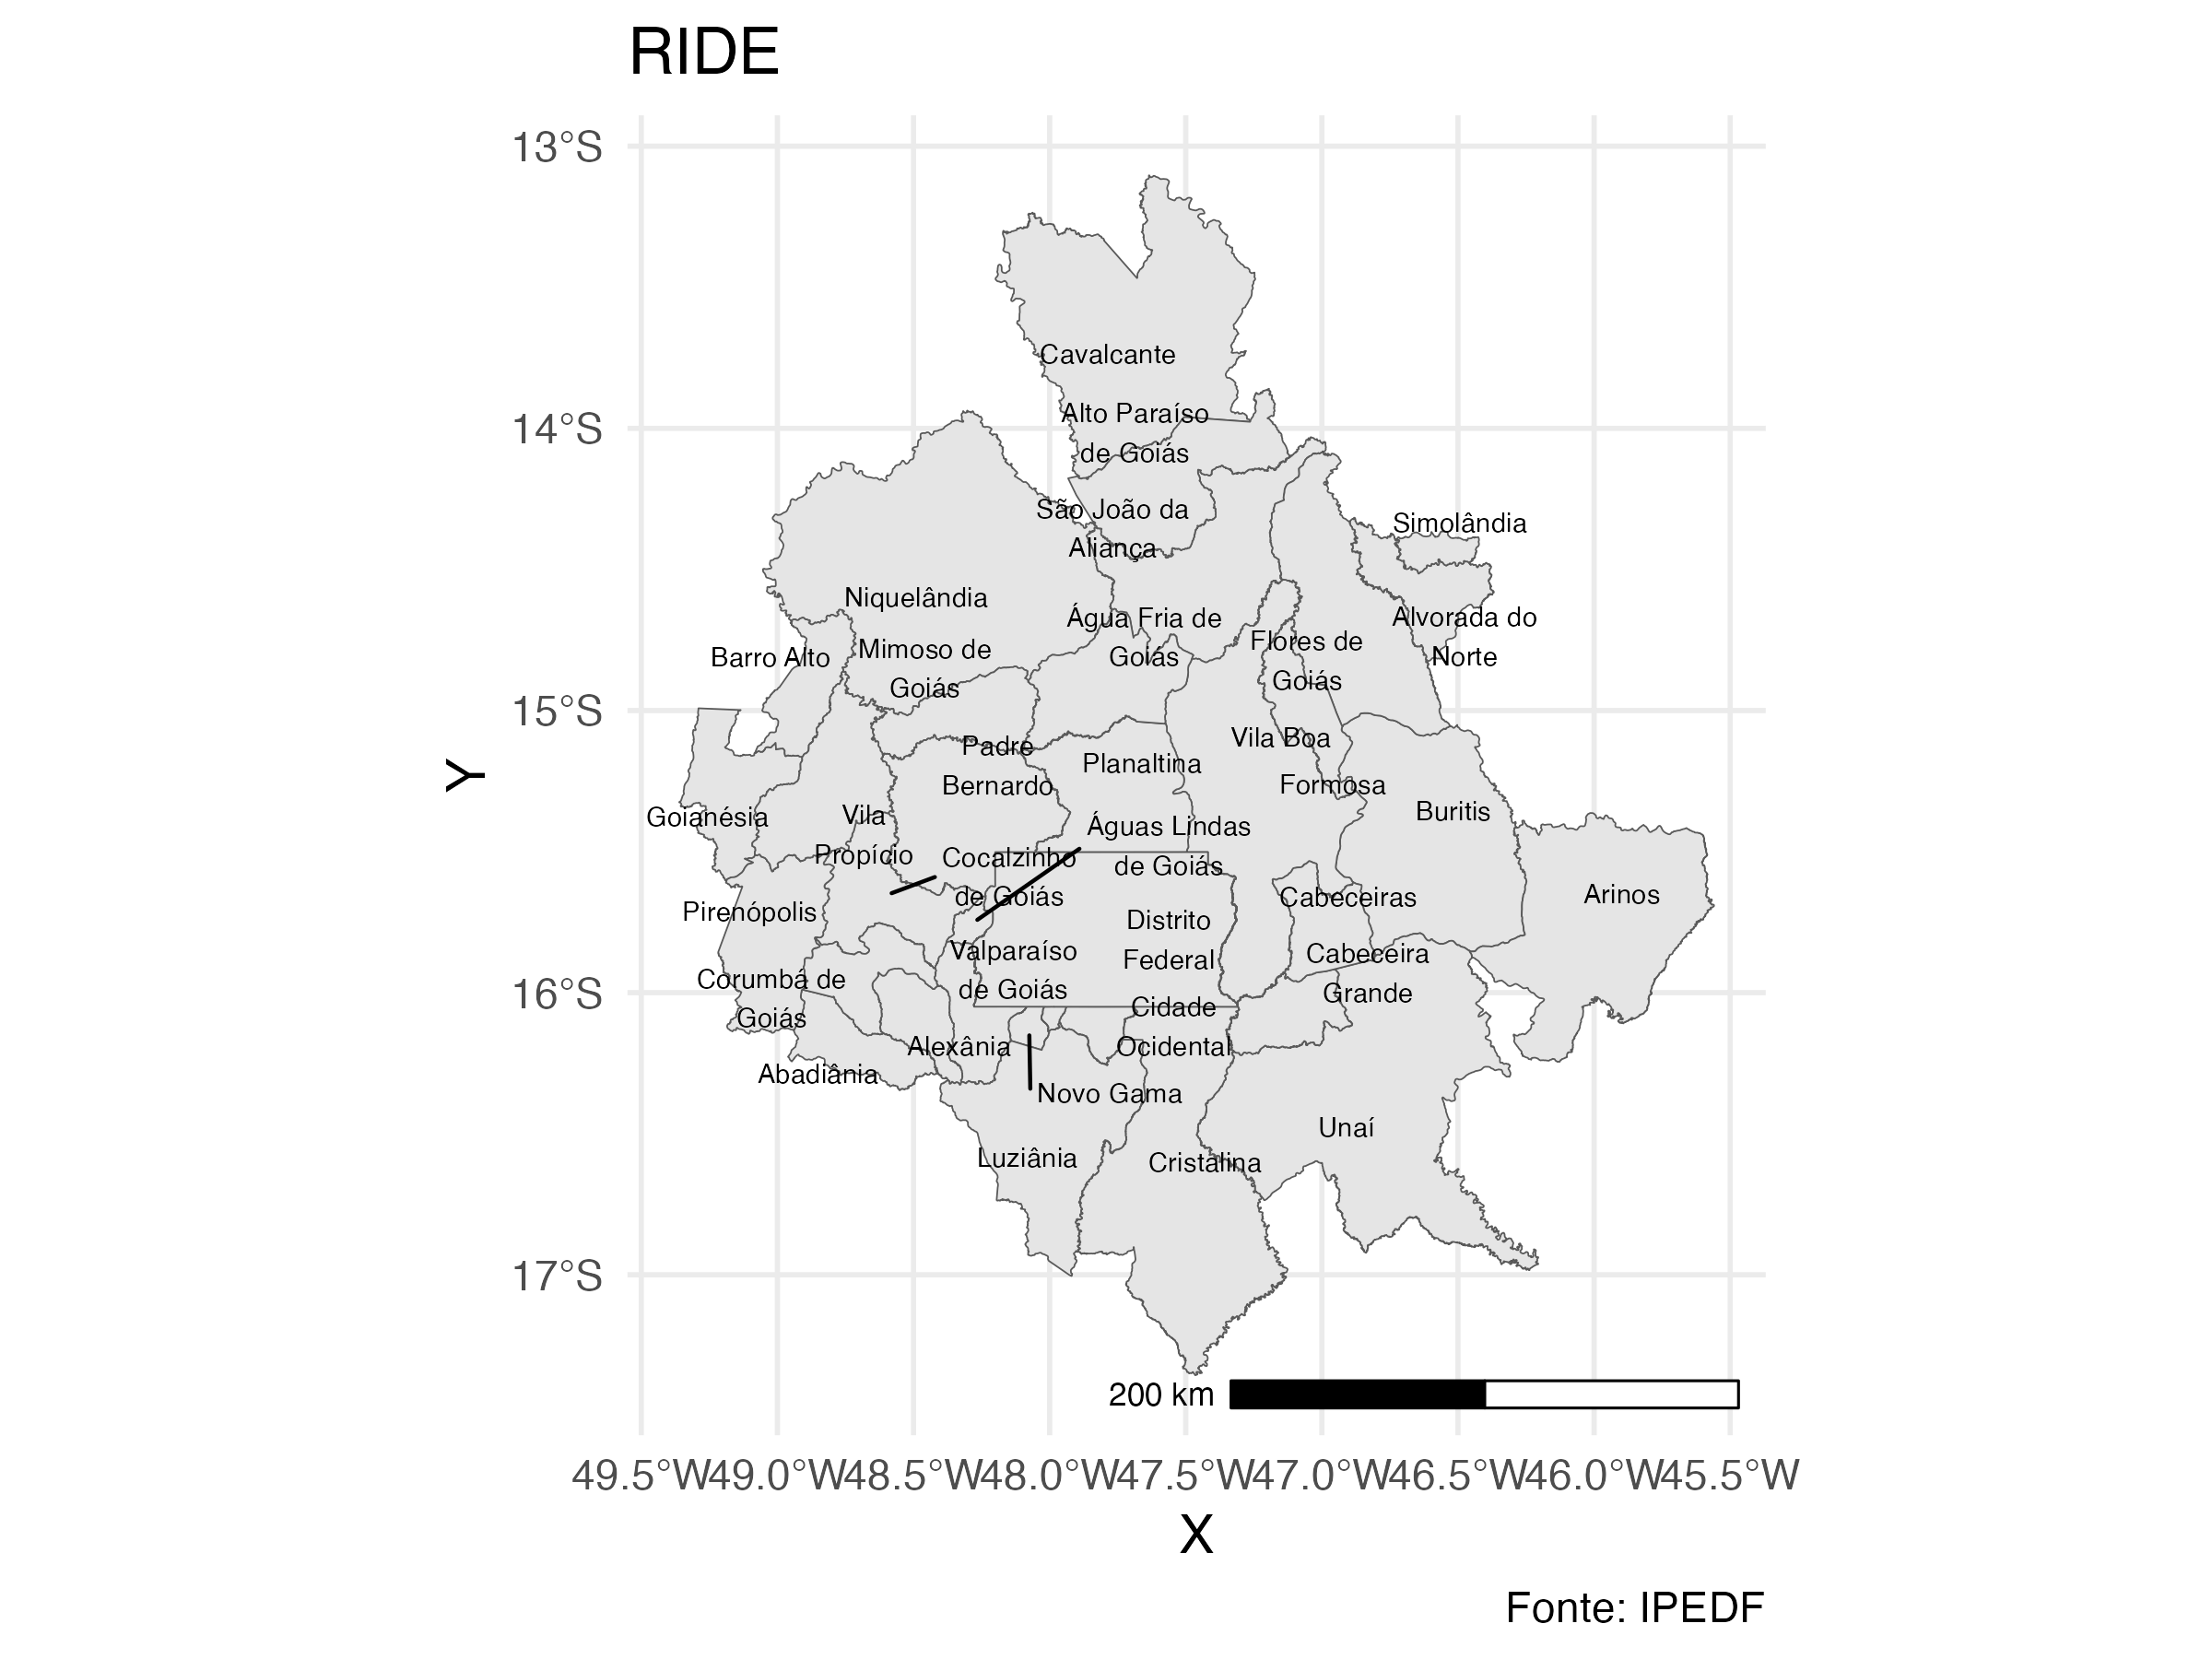
\includegraphics[width=8in,height=\textheight]{ride.png}

}

\caption{\label{fig-mapa-ride}Municípios que compõem a RIDE (Região
Integrada de Desenvolvimento do DF e Entorno).}

\end{figure}%

\subsection{Material e Métodos}\label{sec-data-methods}

Para a obtenção dos dados de temperatura utilizados neste trabalho,
recorreu-se à plataforma Earthdata, mantida pela NASA em parceria com o
Serviço Geológico dos Estados Uniddos (USGS), que disponibiliza produtos
de sensoriamento remoto derivados do sensor MODIS (Moderate Resolution
Imaging Spectroradiometer), a bordo dos satélites Terra e Aqua (Wan e
Dozier 2002; NASA Earthdata 2024).

Foi utilizada uma coleção diária de temperatura da superfície terrestre
(Land Surface Temperature -- LST), registrada no período diurno,
aproximadamente às 10h30 no horário local, com resolução espacial de 1
km². Essa variável representa a temperatura radiativa da superfície da
Terra, estimada a partir da emissão térmica captada pelos sensores
MODIS. Os dados são originalmente fornecidos em kelvin e foram
convertidos para graus Celsius para facilitar a análise e a
interpretação. A data selecionada foi 22 de outubro de 2020, coincidindo
com o aniversário da autora e escolhida como eixo temático do estudo.

A área de interesse corresponde à Região Integrada de Desenvolvimento do
Distrito Federal e Entorno (RIDE-DF), composta pelo Distrito Federal por
34 municípios de seu entorno, sendo 30 localizados no estado de Goiás e
4 em Minas Gerais, conforme estabelecido pela legislação federal
vigente. Para delimitar essa região, foi utilizado um polígono
geográfico de referência com abrangência compatível com os limites da
RIDE. Os dados de temperatura foram então recortados com base nesse
polígono, de forma a manter apenas os pontos efetivamente situados
dentro da área de estudo.

No total, foram utilizados 181 medições . As coordenadas dos pontos de
temperatura foram obtidas tanto em formato geográfico (latitude e
longitude) quanto em sistema projetado UTM (Universal Transverse
Mercator, zona 23S, SIRGAS 2000), sendo este último utilizado nas
análises geoestatísticas por ser mais adequado ao cálculo de distâncias
em metros.

\phantomsection\label{cell-fig-pontos-amostrados}
\begin{figure}[H]

\centering{

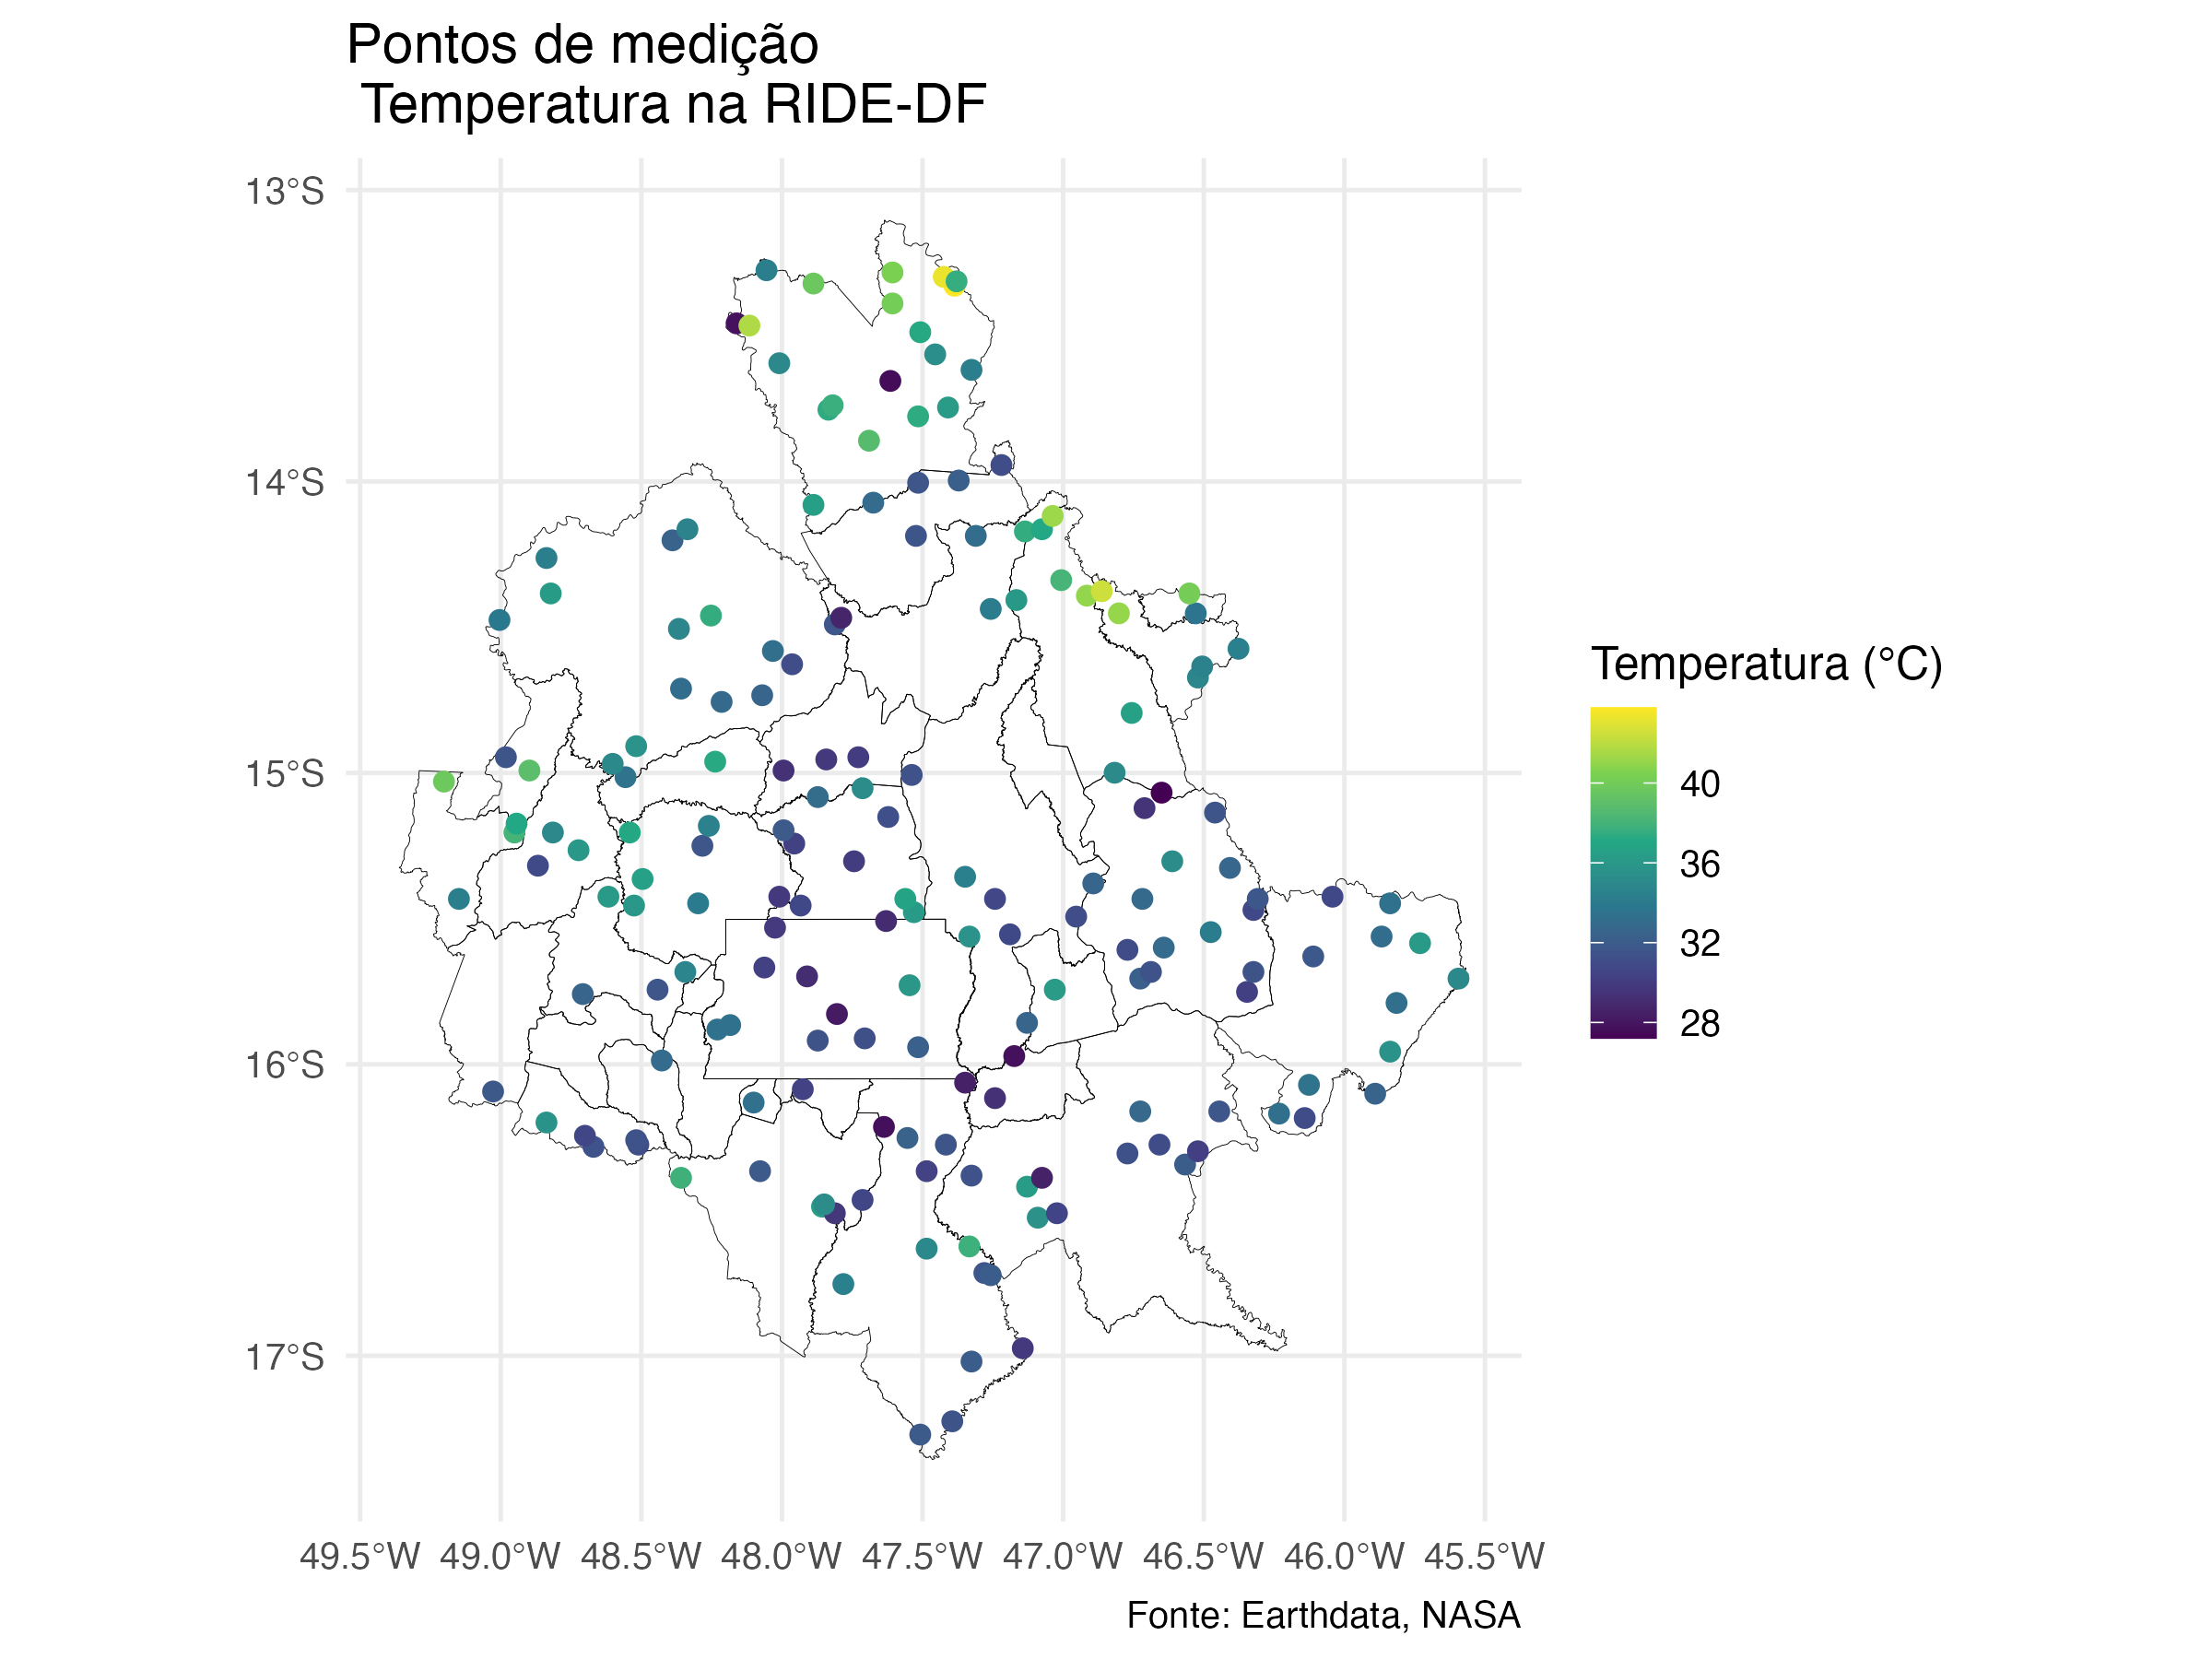
\includegraphics[width=8in,height=\textheight]{ride_temp_points.png}

}

\caption{\label{fig-pontos-amostrados}Pontos amostrados de temperatura
da superfície terrestre (°C) na RIDE-DF.}

\end{figure}%

Com os dados preparados, procedeu-se à aplicação da krigagem ordinária,
técnica de interpolação espacial baseada na teoria dos processos
estocásticos estacionários, que utiliza a estrutura de autocorrelação
espacial da variável observada para gerar estimativas em pontos não
amostrados.

\subsection{Resultados}\label{resultados}

A fim de estimar a temperatura da superfície terrestre em locais não
amostrados dentro da RIDE-DF, foi realizada a modelagem do variograma
empírico com base na amostra dos 181 pontos. Para isso, foram testados
diferentes modelos teóricos de variograma, esférico, gaussiano,
exponencial e linear, com diferentes valores de sill, range e nugget com
o objetivo de avaliar qual estrutura de dependência espacial melhor se
ajustava aos dados.

A comparação visual dos ajustes ( Figura~\ref{fig-ajuste-variogramas})
mostrou que os modelos esférico e exponencial foram capazes de capturar
razoavelmente bem a tendência observada no variograma empírico. O modelo
gaussiano não se ajustou bem quando os dados atingiam o range e o modelo
linear apresentou instabilidades no processo de ajuste, com alerta de
singularidade, e foi descartado da análise final. O gráfico resultante
mostra a semivariância média dos pares de pontos em função da distância
que os separa, evidenciando o grau de dependência espacial da variável.

O modelo exponencial foi selecionado para as análises de krigagem, por
apresentar o melhor compromisso entre aderência visual ao variograma
empírico, simplicidade de interpretação e estabilidade numérica no
ajuste. Conforme discutido por Moraga (2022), esse modelo é
especialmente útil quando a correlação espacial decresce suavemente com
a distância, o que foi observado nos dados analisados.

Com o modelo exponencial ajustado, foi realizada a krigagem ordinária
sobre uma grade regular de pontos com espaçamento de 1 km dentro da área
da RIDE. O resultado foi a geração de uma superfície contínua de
temperatura estimada, representando a variação espacial da LST em toda a
região no dia 22 de outubro de 2020.

\phantomsection\label{cell-fig-ajuste-variogramas}
\begin{figure}[H]

\centering{

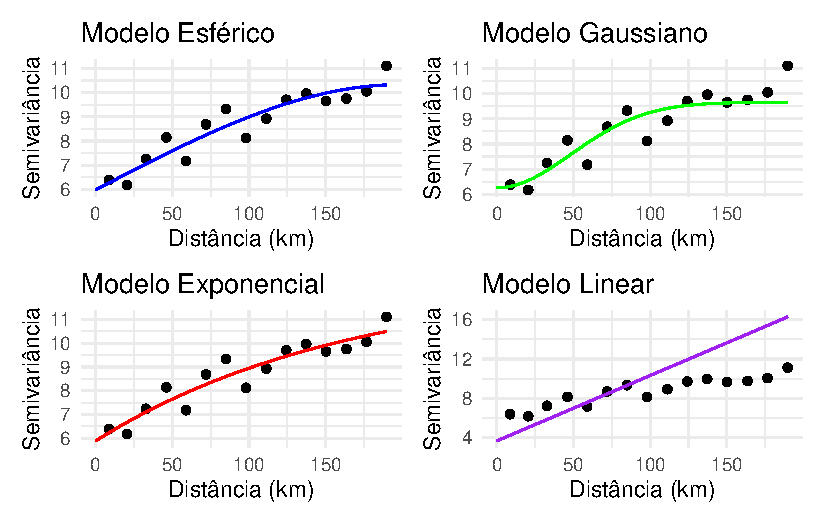
\includegraphics{index_files/figure-pdf/fig-ajuste-variogramas-1.pdf}

}

\caption{\label{fig-ajuste-variogramas}Comparação de modelos de
variograma ajustados aos dados de temperatura da superfície terrestre na
RIDE-DF.}

\end{figure}%

Na sequência, foi ajustado um modelo teórico exponencial, com parâmetros
iniciais definidos para o patamar (sill), efeito pepita (nugget) e
alcance (range). O ajuste obteve convergência e mostrou boa aderência
visual ao variograma empírico, respeitando a tendência de crescimento
rápido da semivariância para pequenas distâncias, característica
compatível com esse tipo de modelo.

O modelo ajustado estimou um nugget de aproximadamente 3, indicando uma
parcela de variabilidade que não é explicada pela estrutura espacial,
possivelmente atribuída a erros de medição, microvariações locais ou
ruído do processo. O sill (patamar da variância total) foi estimado em
torno de 15, valor que representa o nível de estabilização da
semivariância para distâncias maiores. Já o range foi estimado em cerca
de 150 km, sugerindo que pontos distantes até essa ordem de magnitude
ainda apresentam correlação espacial significativa.

Esses valores são consistentes com um cenário em que a temperatura de
superfície apresenta autocorrelação espacial de média escala, com
variação gradual ao longo do território da RIDE, o que justifica o uso
da krigagem como interpolador.

\begin{verbatim}
[using ordinary kriging]
\end{verbatim}

Para a aplicação da krigagem, foi construída uma grade regular de
predição sobre a área da RIDE, com espaçamento de 2.500 metros entre os
pontos centrais. Esse valor foi escolhido com o objetivo de manter boa
resolução espacial ao mesmo tempo em que se preserva a legibilidade
visual da trama da grade. Os pontos da grade foram filtrados para
incluir apenas aqueles contidos dentro dos limites geográficos da região
de estudo.

A Figura~\ref{fig-grade-krigagem} apresenta os pontos da grade de
predição (em vermelho) distribuídos de forma homogênea ao longo da RIDE,
além dos pontos amostrados utilizados para o ajuste da krigagem. Estes
pontos amostrados estão representados por marcadores pretos,
acompanhados dos respectivos valores de temperatura da superfície
terrestre (em graus Celsius).

\phantomsection\label{cell-fig-grade-krigagem}
\begin{figure}[H]

\centering{

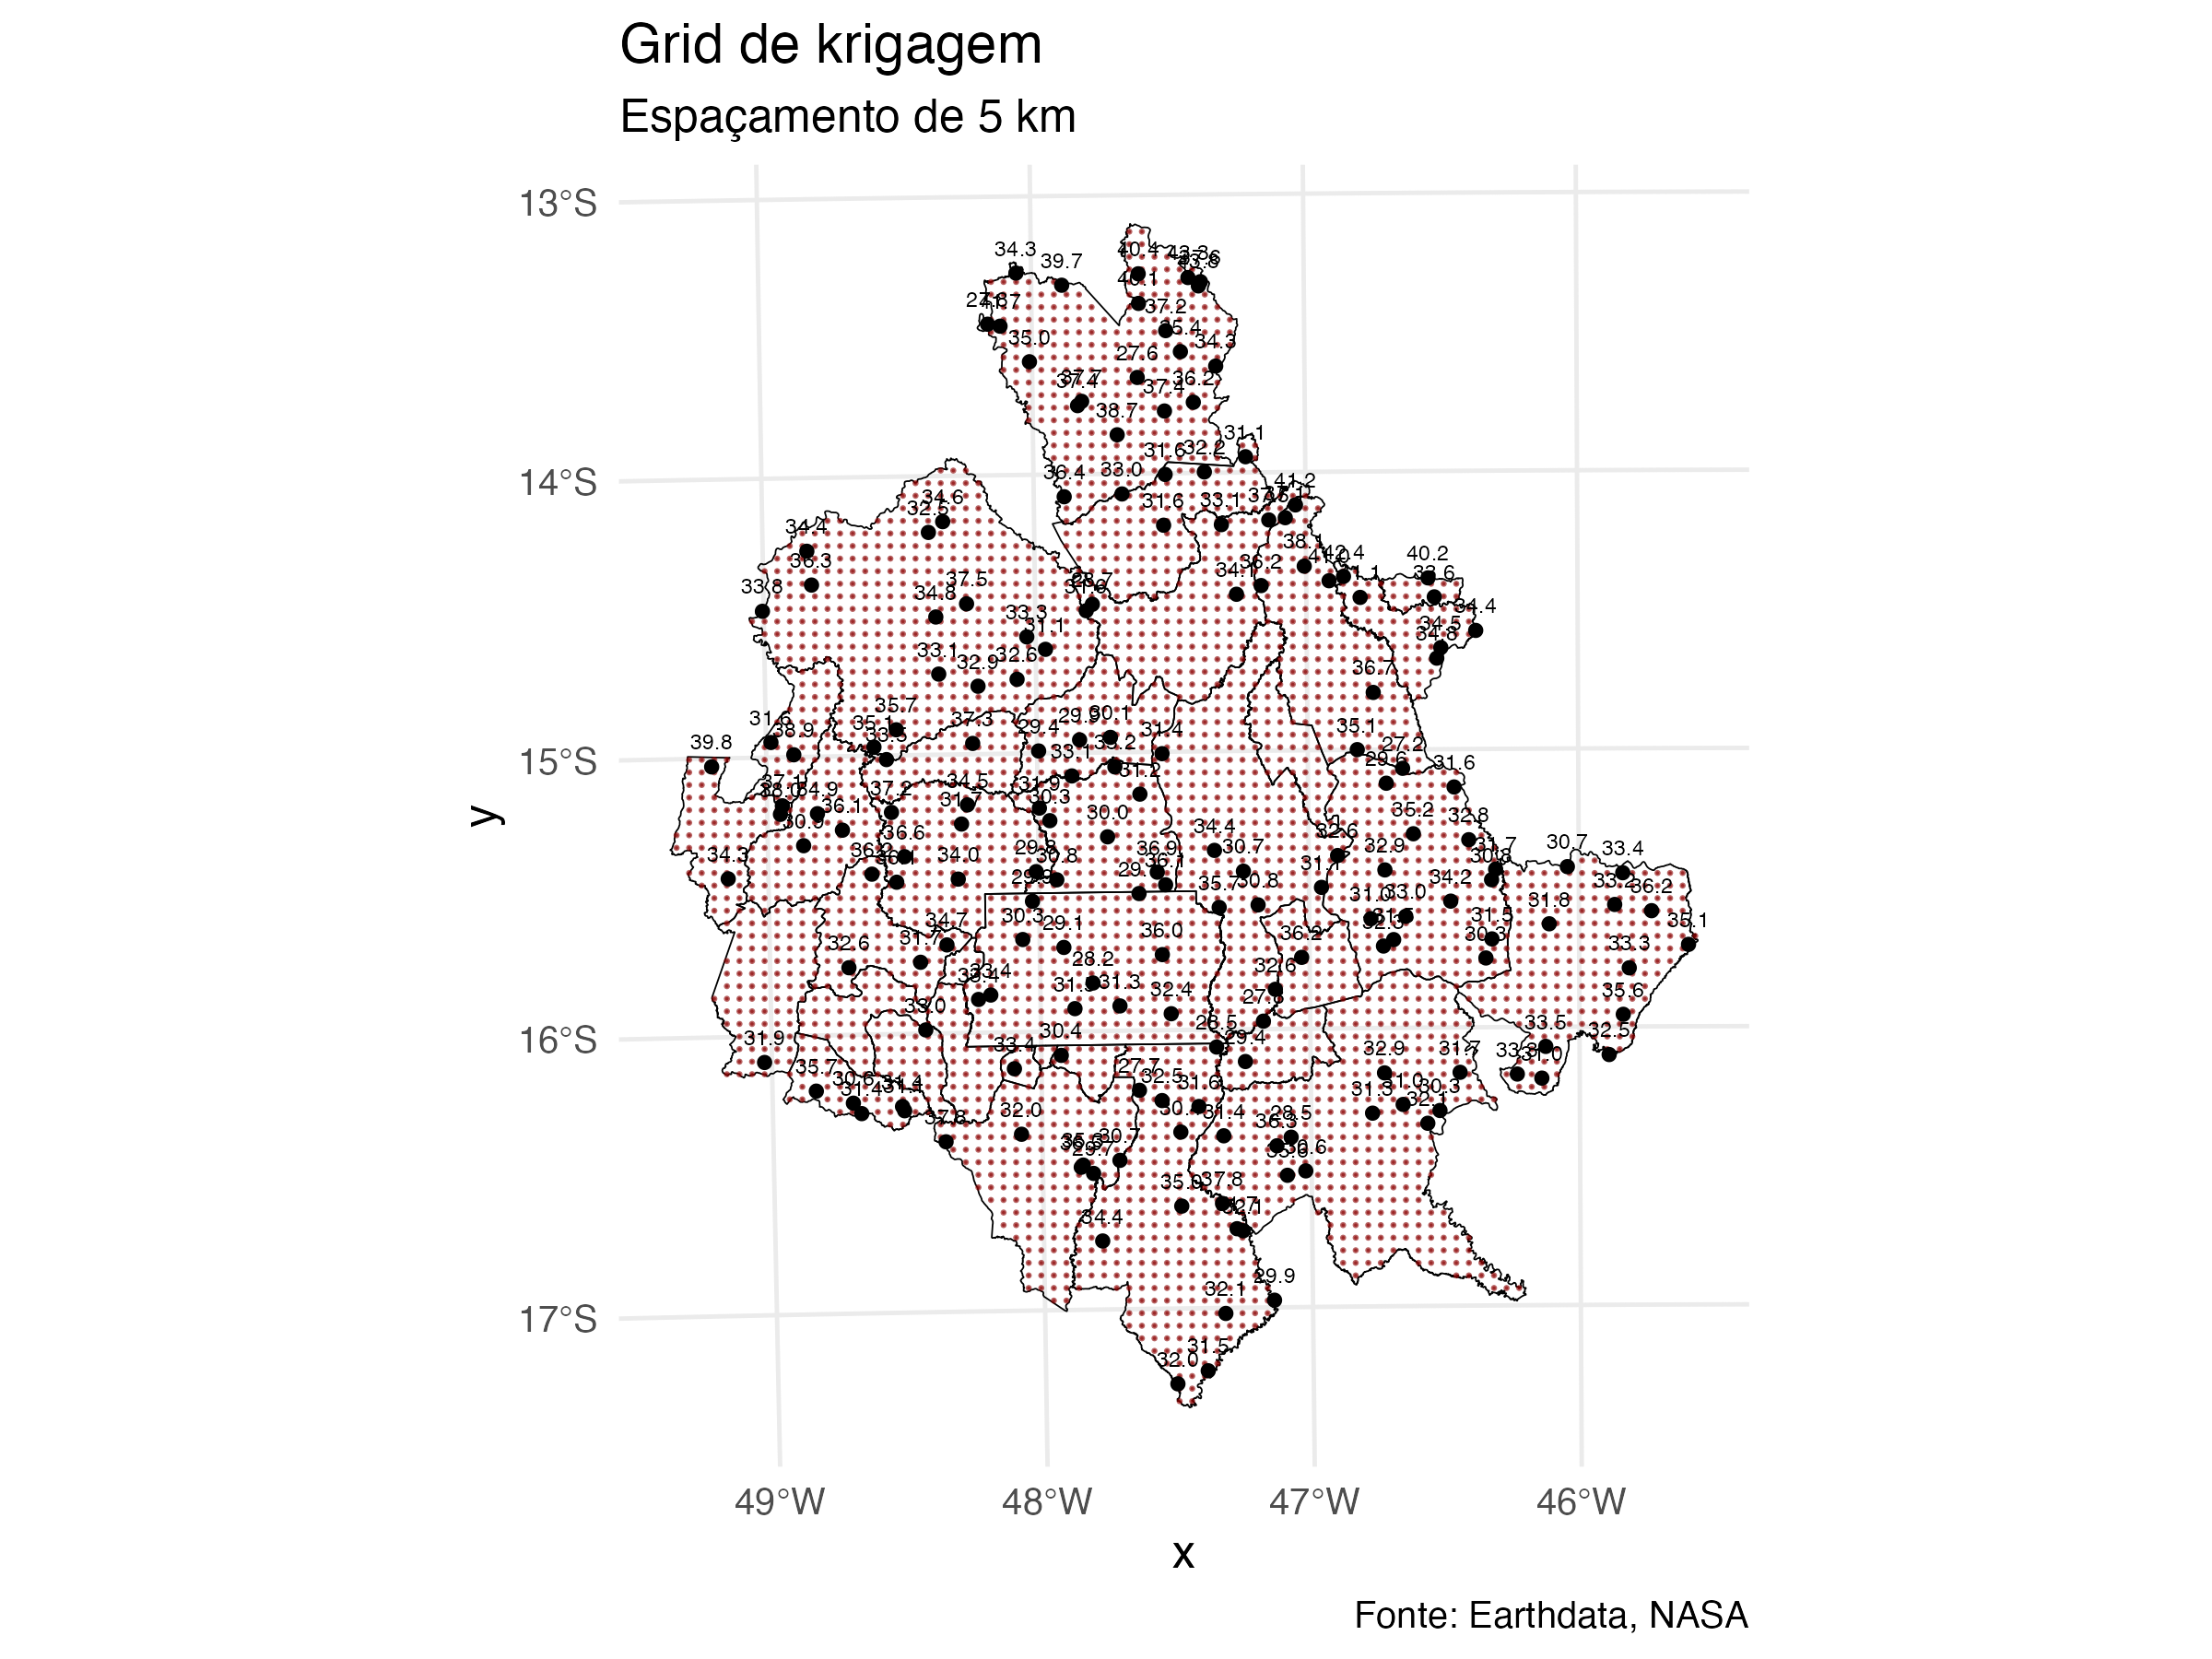
\includegraphics[width=8in,height=\textheight]{ride_temp_grid.png}

}

\caption{\label{fig-grade-krigagem}Grid predição (2,5 km) e pontos com
temperatura observada.}

\end{figure}%

\begin{verbatim}
[using universal kriging]
\end{verbatim}

Além da krigagem ordinária, foi também aplicada a krigagem universal,
que considera a presença de uma tendência espacial global na média da
variável de interesse. Nesse caso, admitiu-se que a temperatura da
superfície terrestre poderia variar de forma sistemática ao longo do
espaço, e essa tendência foi modelada por meio das próprias coordenadas
UTM (x e y) dos pontos de amostragem.

O modelo ajustado incorporou essa estrutura, permitindo estimar a média
da temperatura como uma função linear das coordenadas espaciais,
enquanto a dependência residual foi tratada pela estrutura variográfica
previamente ajustada.

Apesar da incorporação dessa estrutura adicional no modelo, a comparação
visual entre os mapas resultantes da krigagem ordinária e da krigagem
universal ( Figura~\ref{fig-krigagem-comparacao}) não revelou diferenças
perceptíveis na superfície interpolada. Ambas as abordagens produziram
mapas semelhantes, com padrões espaciais suaves e coerentes com a
distribuição dos dados observados.

Essa ausência de distinção visual pode ser explicada por características
da própria área de estudo: a RIDE-DF está localizada em uma região de
relevo relativamente plano e contínuo, com uma distribuição espacial de
temperatura que, ao menos na data considerada, não apresenta gradientes
acentuados ou tendências marcantes ao longo das coordenadas geográficas.
Em contextos assim, a contribuição de uma estrutura de tendência global
tende a ser pequena, fazendo com que a krigagem universal e a ordinária
produzam resultados semelhantes.

\phantomsection\label{cell-fig-krigagem-comparacao}
\begin{figure}[H]

\centering{

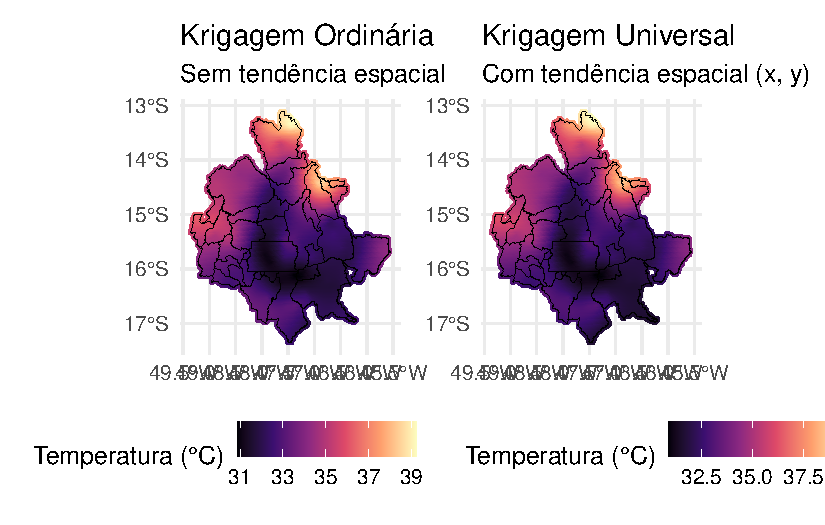
\includegraphics{index_files/figure-pdf/fig-krigagem-comparacao-1.pdf}

}

\caption{\label{fig-krigagem-comparacao}Superfícies de temperatura
estimadas por krigagem ordinária (à esquerda) e universal (à direita) na
RIDE-DF. Ambas apresentam padrões espaciais semelhantes, refletindo a
distribuição dos dados observados.}

\end{figure}%

Avaliando a superficie de erros vemos que os erros sao menores perto dos
posntos amostrados como esperado lalala

Avaliando a superfície do erro padrão das predições por krigagem
(Figura~\ref{fig-superficie-erro-padrao}), observa-se que os menores
valores de incerteza concentram-se nas regiões próximas aos pontos de
amostragem, como era esperado. Nessas áreas, a densidade de informação
observada permite ao modelo realizar predições mais confiáveis,
reduzindo a variância associada. Por outro lado, nas porções mais
periféricas da RIDE, especialmente em trechos do norte, nordeste e
extremo oeste ---, os valores do erro padrão se elevam, refletindo a
maior distância em relação aos dados utilizados no ajuste da krigagem.

Esse comportamento é característico do método geoestatístico adotado,
uma vez que a precisão da predição decai com o aumento da distância em
relação aos pontos observados. Além disso, nota-se que tanto a krigagem
ordinária quanto a universal apresentaram padrões similares de erro
padrão, reforçando a conclusão de que a inclusão da tendência espacial
não resultou em ganhos substantivos de acurácia no presente contexto.

\phantomsection\label{cell-fig-superficie-erro-padrao}
\begin{figure}[H]

\centering{

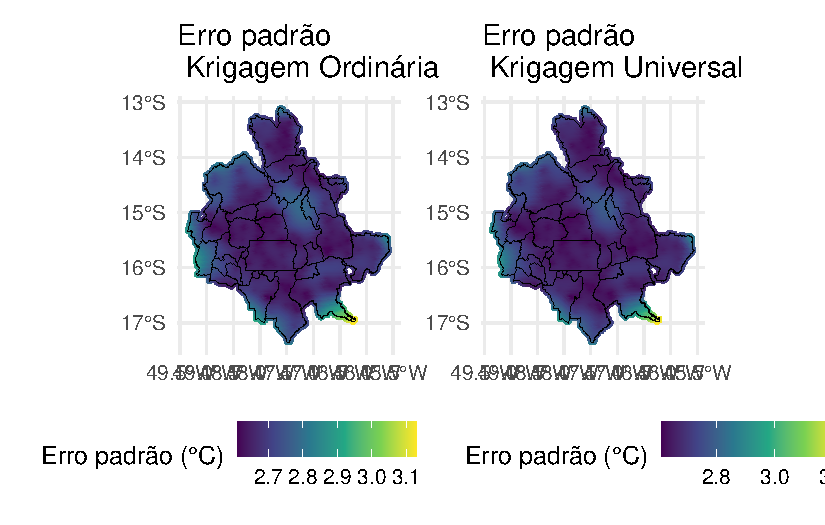
\includegraphics{index_files/figure-pdf/fig-superficie-erro-padrao-1.pdf}

}

\caption{\label{fig-superficie-erro-padrao}Superfície do erro padrão das
predições por krigagem ordinária (à esquerda) e universal (à direita) na
RIDE-DF. Valores mais baixos próximos aos pontos amostrados indicam
maior confiança na interpolação nessas áreas.}

\end{figure}%

\subsection{Conclusões}\label{conclusuxf5es}

A superfície de temperatura estimada pela krigagem revela padrões
espaciais coerentes com as características geográficas e ambientais da
Região Integrada de Desenvolvimento do Distrito Federal e Entorno
(RIDE-DF). Observa-se uma tendência de temperaturas mais elevadas nas
porções norte e oeste da região, especialmente em municípios como
Cavalcante, Alto Paraíso de Goiás, Niquelândia e Barro Alto. Essas
localidades são marcadas por altitudes relativamente mais baixas,
presença predominante de áreas abertas, pastagens e agricultura
extensiva, e menor cobertura florestal, fatores que favorecem maior
absorção de radiação solar e aquecimento da superfície terrestre
(Moraga, 2022). E eu também por acaso já notei que Cavalcante costuma
ser bem mais quente que Brasília quando vou la acambar no Parque
Nacional da Chapada dos Veadeiros.

Em contraste, as temperaturas mais amenas concentram-se na porção sul da
RIDE, em municípios como Cristalina, Luziânia, Cidade Ocidental e Novo
Gama, além do centro-leste da região, abrangendo o Distrito Federal.
Essa distribuição se alinha à topografia mais elevada do Planalto
Central, onde altitudes frequentemente superam os 1.000 metros,
contribuindo para uma moderação térmica natural. A maior presença de
manchas urbanas contínuas com arborização significativa, aliada a áreas
de proteção ambiental como o Parque Nacional de Brasília, também pode
resultar em temperaturas de superfície mais baixas, configurando, em
alguns trechos, o fenômeno conhecido como ``ilha de frescor urbano''

Os dados utilizados referem-se à temperatura da superfície terrestre
(Land Surface Temperature -- LST) captada via sensoriamento remoto no
período diurno (\textasciitilde10h30), sendo sensíveis à cobertura e ao
uso do solo, à umidade superficial e ao relevo. Como a data de
referência é 22 de outubro de 2020, dia do aniversário da autora, e
também um dos mais quentes daquele ano na região ---, a escolha do
recorte temporal não foi apenas afetiva, mas também climática. Trata-se
de um momento de transição entre a estação seca e o início da estação
chuvosa no Centro-Oeste, período marcado por altos índices de radiação
solar e baixa umidade do solo.

Curiosamente, embora a memória térmica da autora guarde a Asa Norte como
um forno reformando sem ar-condicionado, os dados mostram que havia
regiões significativamente mais quentes na RIDE naquele dia. Assim, o
sofrimento era real, mas não estava sozinho: a superfície do Planalto
queimava de forma coletiva

\subsection*{Referências}\label{referuxeancias}
\addcontentsline{toc}{subsection}{Referências}

\phantomsection\label{refs}
\begin{CSLReferences}{1}{0}
\bibitem[\citeproctext]{ref-earthdata}
NASA Earthdata. 2024. {«Earthdata Search»}.
\url{https://search.earthdata.nasa.gov}.

\bibitem[\citeproctext]{ref-wan2002modis}
Wan, Zhengming, e Jeff Dozier. 2002. {«MODIS land surface temperature
products»}. \emph{Remote Sensing of Environment} 83 (1-2): 163--80.

\end{CSLReferences}



\end{document}
